
\subsection{The Segway System}
The segway was constructed using a metal plate as foundation for the robot.
The motors were then attached to the lower side of the plate.
On top of the basis was then mounted the PCB designed with the two H-bridges to control the two motors.

A second layer was then added as a plug-in module to which the different components could be plugged in and on which the power supply circuit is, converting the input voltage to a 5V supply for the FPGA.
This layer included a plug for the FPGA and the IMU.
Furthermore was there added plugs for a bluetooth sender/transmitter and two wheel encoders, but due to time constraints was it chosen not to use their functionality since it was not required for the system to work at the given state.

A sketch of the final segway is seen in figure \ref{fig:segwaysketch}.

\begin{figure}[H]
\centering
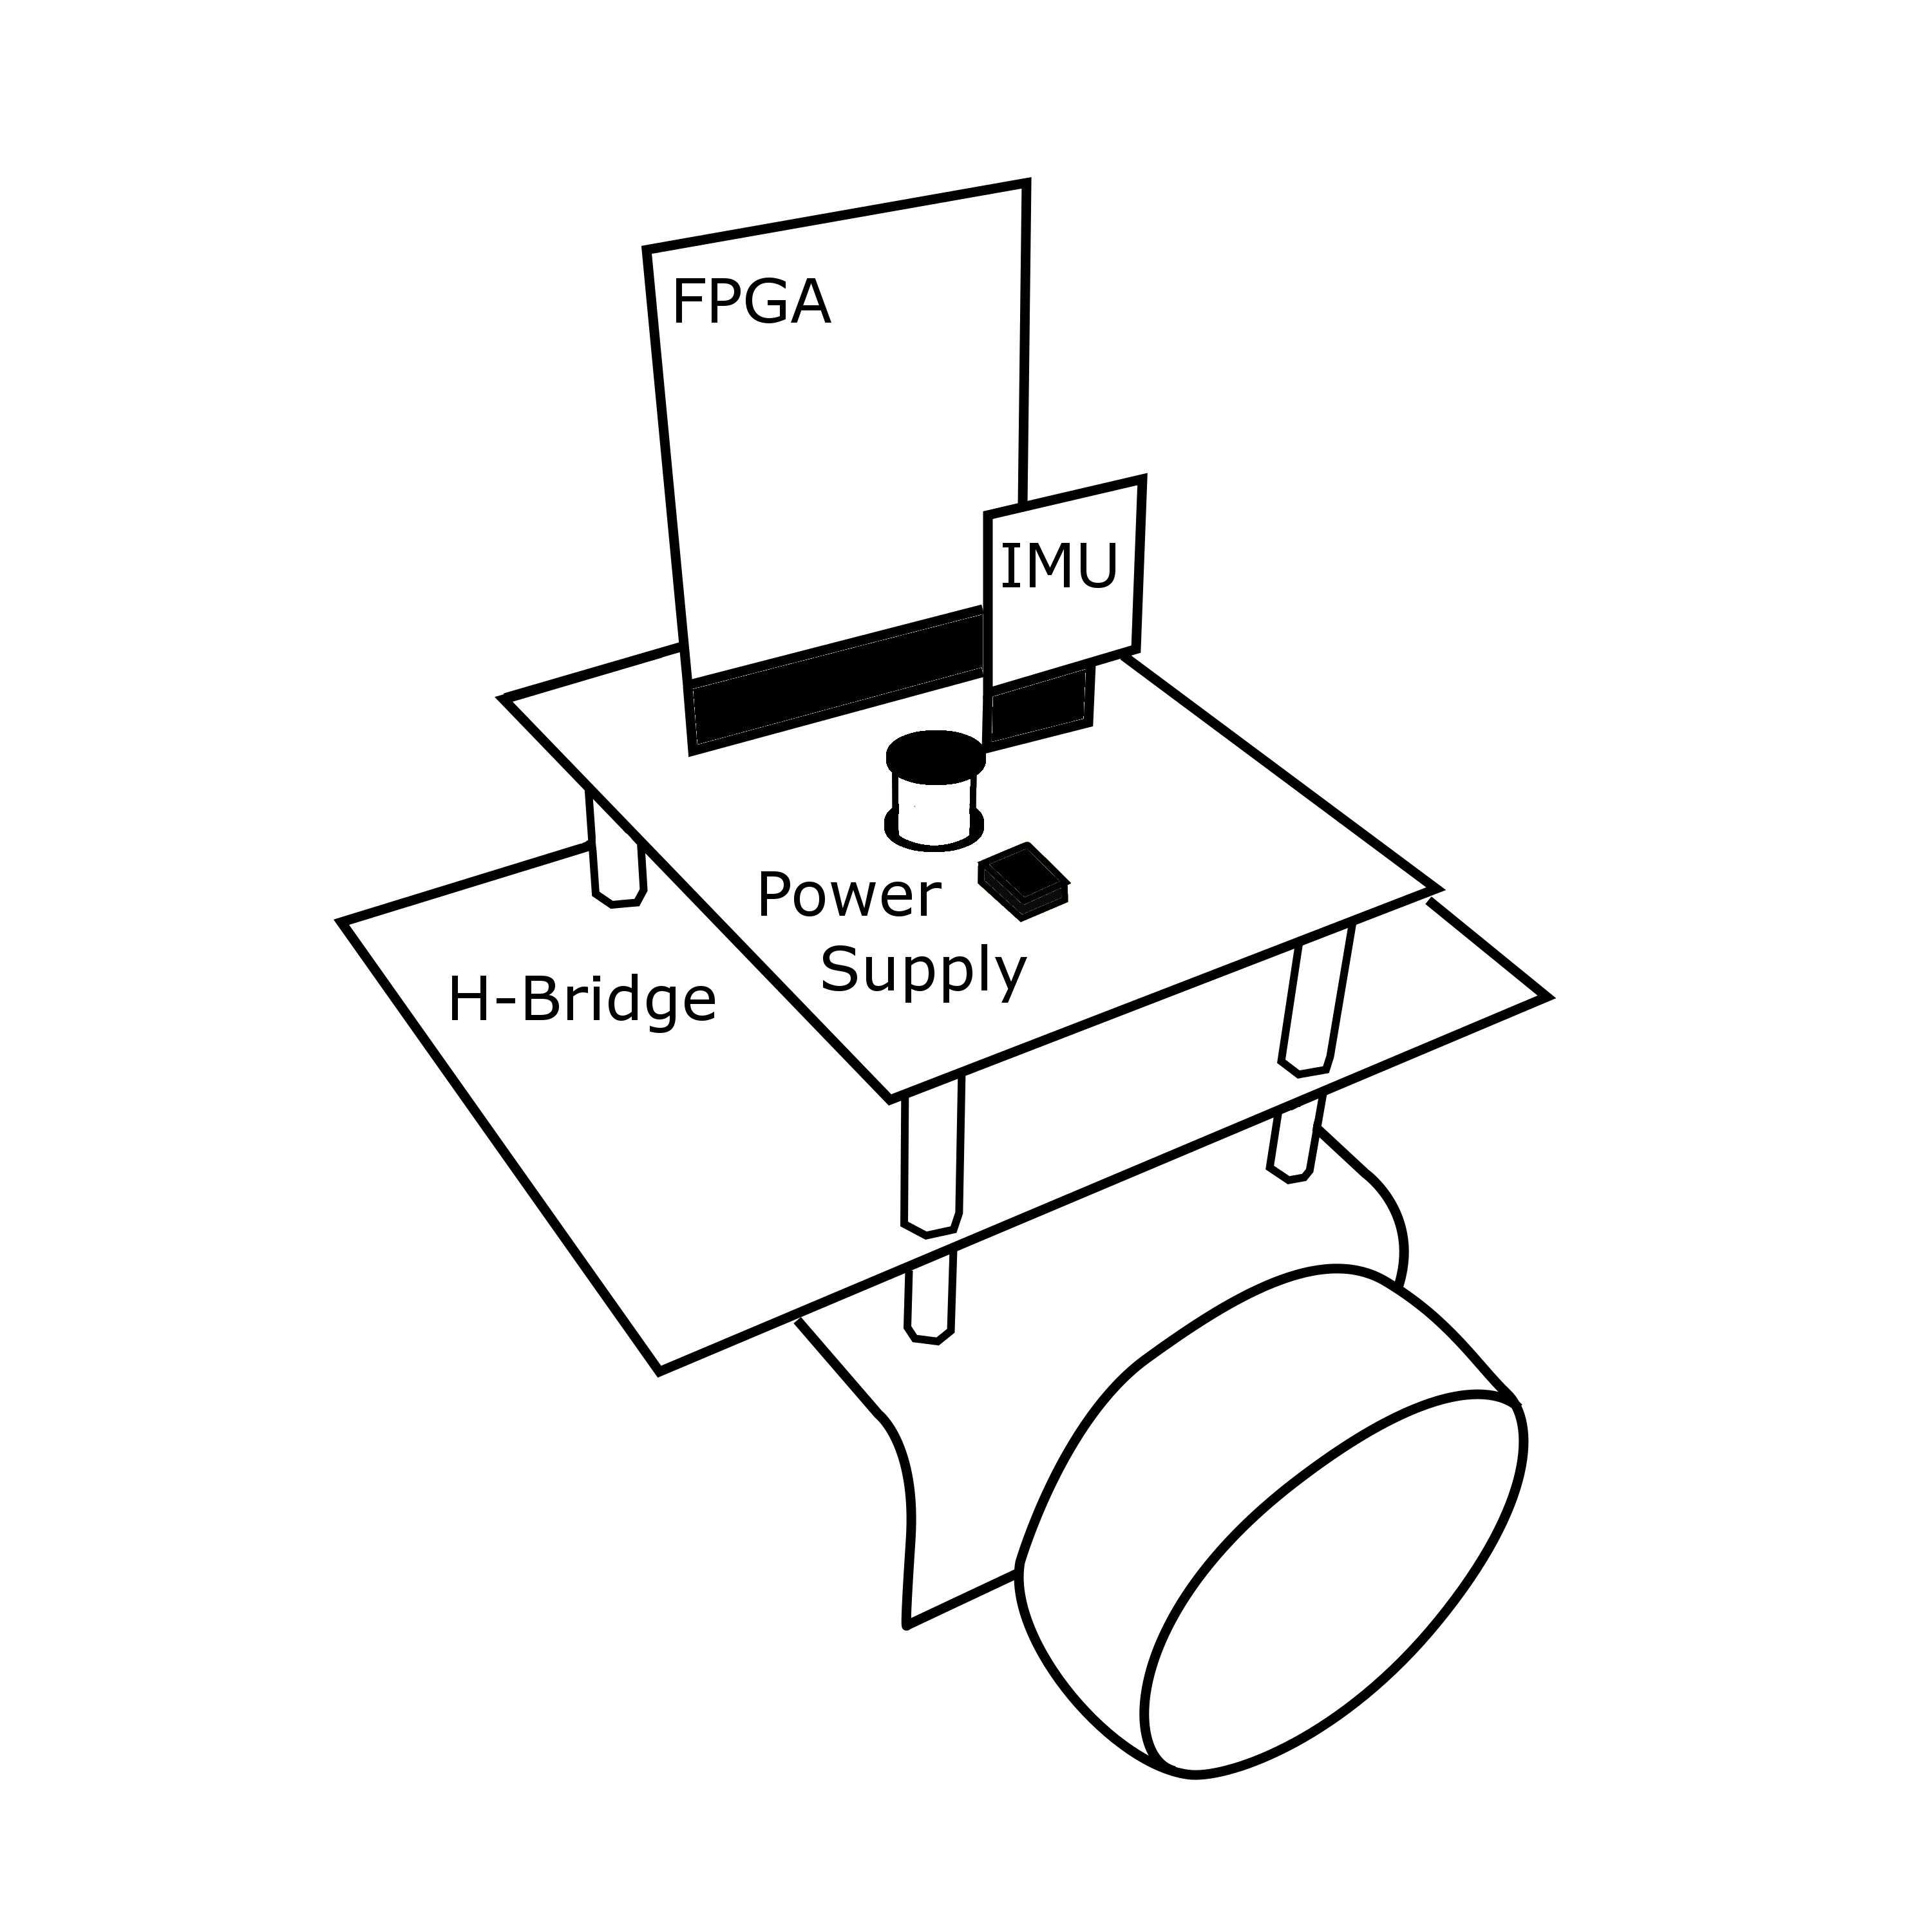
\includegraphics[width = 0.5 \textwidth]{images/segway}
\caption{Sketch of the build segway.}
\label{fig:segwaysketch}
\end{figure}

As seen on figure \ref{fig:segwaysketch}, then the goal of the final segway design was to center the center of mass above the wheel axis when the segway stands in upright position.
This was done by using mirrored design, where possible, when designing the boards and center the FPGA and other electronics about the same axis.
